% Implementation (4000 words)
% * Refer to design strategies that looked ahead to the testing stage
% * Draw attention to what is not my own work (ie rebar, webmachine etc)
% * Major milestones might be highlighted with advantage
% *! Show evidence of skill, clear thinking and common sense

% ************
% Should have: 
% 	intro
% 	content
% 	summary
% ************

% Word budget 4000 words. Try to keep it less
\section{Implementation}

In this chapter I will briefly discuss what data is stored in the Distributed Hash Tables, and also how I get around the problem of efficiently searching through a key-value store and how the changes made to allow this affect the overall performance of the system.

We will then look at what third party libraries are part of the code base, how test-driven development played a crucial part in the development of my project and then go on to look at the high level components that make up the system.

Finally we will discuss how Distributed Hash Tables operate, and more interestingly what distinguishes Chord and Pastry from each other, before we look at how the Erlang concept of process supervision helped me develop a modular and fault tolerant system.

% Content
%   What is to be stored
%     How do we solve search across key's?
%     How much space does this take up?
%       Average name length?
%       Amount of data per user?

\subsection{General discussion}
Before I start discussing how I implemented my project, I want to discuss what data I am interested in storing in my search network, and how I built a search index on top of a distributed hash table. 

\mbox{}

My search network stores records with information about users, much like a normal address book does. I made the following fields mandatory: the person's name, a url to her online social network profile page, and a url to a profile image that can be displayed alongside the search result.

For the purpose of this project I did not want to lock down exactly what data should be stored, but before my system is used in a wider context it would be wise to look into using some well known public standard. At this stage it is outside the scope of my project.

As I briefly discussed in the preparation chapter, a key-value store does not immediately lend itself to search. If you don't know the key under which a data item is stored, you would have to do a linear search across the keyspace in order to find what you are looking for. 

The solution is to use the persons name as the key. Human names in their natural form do not easily map uniformly onto any linear keyspace. They are of different length and also cluster around more common names. I therefore used a hashing function to hash names into keys. This immediately presents us with another problem. If you don't know the exact spelling of the name that was used to generate the key you still can't get around a linear search through the datastore. You can partly solve this problem by normalising names before hashing them into keys, but the utility of a search engine that requires you to already know a complete and correct match of what you are looking for is arguably rather low. Users today increasignly expect search engines to deliver predictive searches where results show before you finish typing your search query. This scheme does neither accommodate this, nor does it misspelled names, or for that matter cases where you have forgotten your friends middle name.

I solved the problem in the following way: Instead of storing just profile records I store both \emph{profile records} and \emph{link records}. The profile records contain all the information stored about a user in the system, and are accessible under a key generated by hashing the whole record. The link records on the other hand are lightweight pointers to the full profile records. They contain the full name and the key of the profile record, and are stored under a key generated by a subset of the users full name. Each profile record has multiple link records pointing to it. I will come back to how I am generating these link records shortly.

Using link records solves several problems. By storing links keyed by fragments of a users name, the search engine can start looking up information before the user has completed typing the search phrase. This enables predictive search. Since the link records also contain the full name of the user you can detect and work around misspelled names, or even searches that don't include all the users names.

% How link records are generated
\begin{figure}[!htb]
\begin{center}
	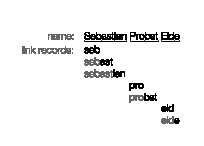
\includegraphics[width=0.6\linewidth]{illustrations/LinkRecords.eps}
  \caption{Here it is shown how a name maps into name fragments used for storing link records pointing to a profile record.}
  \label{figLinkRecord}
\end{center}
\end{figure}

In the current implementation I create link records for each three additional characters contained in a users name. This is illustrated in figure \ref{figLinkRecord}. The process is done separately for each name. Initially the first three characters of a name are taken. Then for the next link records key the subsequent three characters are added. This process is repeated until you reach the end of a name. When you reach the end of a name that is not a multiple of 3, an additional link record is created for the full length of the name. In the example in figure \ref{figLinkRecord} you see this illustrated in how Eide results in the link records \emph{eid} and \emph{eide}.

Using link records does generate extra overhead when searching. A search will now no longer require a single lookup in the search index, but several. As the user types the search server will have to look up link records and resolve them to their profile records. If you searched for my full name, a total of 9 requests would have to be made. 8 for each of the link entries, and an additional one for looking up the full record with all the information about the user. 

In reality it isn't quite as bad as it sounds. The desired result is likely to show up before the user has finished typing, in which case lookups for the remaining link items won't be necessary.

The link items also let the search server rank results by relevance. Let me illustrate this with another example. Say the system contains two profile records: one for Probst and one for Probstonius. If you search for Probst you get two link records, one for \emph{pro} and one for \emph{probst}. Both will return pointers to the profile records of both Probst and Probstonius. Since Probst is a complete match for the search term \emph{probst} while Probstonius is only a partial match, the result for Probst can be given a higher relevance score. The current implementation does this.

The approach of using link records does not come for free. It increases both the amount of data stored per record and also the number of lookups needed in order to find a profile record. I now want to discuss exactly to what extent these parameters are affected.

At my disposal I have a sample of 170 million names from Facebook. While this sample might not entirely accurately reflect all the real names of the human population, I would argue that it closely models the names humans are likely to identify themselves by in online social networks.

By sampling 20 million names and calculating how many link records they would generate, I can say with 99$\%$ confidence that a randomly selected name is likely to generate 5.322 $\pm$ 0.001 link records on average and likewise I can say with 99$\%$ confidence that this particular name will be 14.959 $\pm$ 0.002 characters long on average.
Since each link record consists of a users full name, the key of the profile record and its own key, this will result in roughly 2kbit of extra storage assuming 8 bits per character and 160 bit keys. The benefits of getting predictive searches and the ability to handle misspelled and incomplete names in my opinion greatly outweigh the extra storage requirements.

Estimating how many extra lookups result in using link records is significantly more involved. There will be significant amounts of records sharing the same link records for shorter name segments. If one wants to resolve all of these to their respective profile records, a substantial overhead is incurred. TODO: MAKE SOME EDUCATED GUESSES BASED ON DB of NAMES FROM FACEBOOK and PROJECT COST.

%   Parts not my own
%     Rebar build system
%     Webmachine http arbitrator
%     OTP
%       gen_server
%       supervisors

\subsection{Third party code used}
In this section I want to briefly discuss what third party projects I am using in my project.

Most prominent is my dependence on OTP, the Open Telecom Platform, which is part of the Erlang standard distribution. It is a set of libraries that provide basic functionality needed to write amongst others general servers, and provide functionality for supervising processes within your application and restarting them when they fail. Most Erlang applications rely on OTP.

I also used Webmachine, an open source framework for creating HTTP interfaces in Erlang, and a build system called rebar. Both are developed by Basho.

For testing I used EUnit, part of the standard Erlang distribution, for regular functional unit tests and Erlymock for testing functions with side effects where I wanted to control the functions interactions with the environment.


%   Methology
%     Test driven development
%     Integration testing for gen_server
%   Made it modular.
%   Swappable DHT

\subsection{Process}
At this time it is well understood how Distributed Hash Tables work. The bulk of research in Distributed Hash Tables was done around year 2000. The research papers presenting Chord and Pastry also supply high level code that I referenced when implementing the algorithms. This provided an excellent foundation for doing test-driven development. All the core components of my system were unit tested, and in the tradition of test-driven development I started by writing tests and then wrote the minimal code needed to satisfy my tests. This encourages writing modular systems with self-contained and side effect free functions.
I wrote additional integration tests where I felt it served a purpose.

Modularity was also a key design factor for other reasons. I wanted as many as possible of my modules to be ignorant of which Distributed Hash Table was being used. This encouraged me to keep the interface between the Distributed Hash Tables and the surrounding code strict and minimal. In effect the only methods the Distributed Hash Tables needed to export were ways to get and set values by key.


%   Components of the system
%     Client side
%       Backend
%         Controller
%         DHT's
%       Frontend
%         Search server
%         web api
%       How it all fits together
%     Hub side
%       Web API
%       HubController

\subsection{Components of my system}
I now want to describe the design of my system, and how all the different pieces fit together.

My project has two major parts, each its own application. The search application itself, and a hub application that runs at a central, publicly known location. The hub application acts as a rendevouz point for new Chord and Pastry nodes, and is also used to control and initiate experiments.

\mbox{}

I will first discuss the search application itself:


\subsubsection{The Search application}

% Component overview
\begin{figure}[!htb]
\begin{center}
	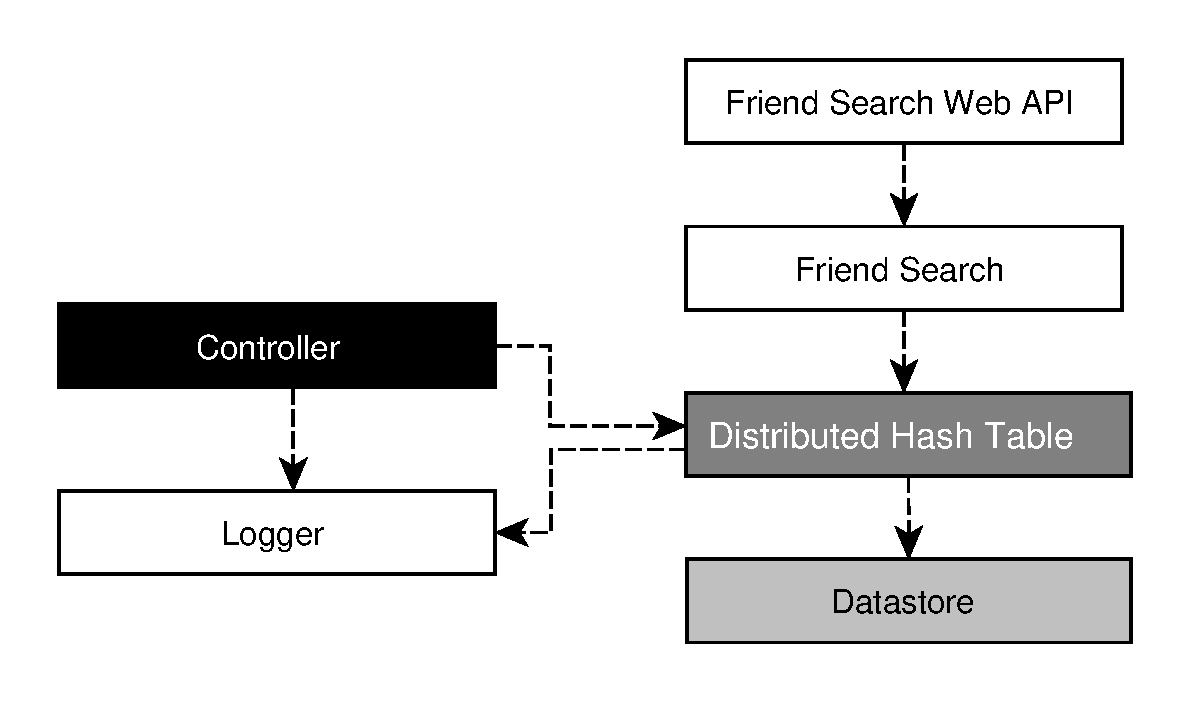
\includegraphics[width=0.9\linewidth]{illustrations/ComponentOverview.eps}
\caption{High level overview of the components of the search application. The arrows show how components interact.}
\label{figComponents}
\end{center}
\end{figure}

Figure \ref{figComponents} shows the main high level components of the search system. I will briefly discuss them in turn:

The \emph{Controller} is the heart of the application. It is the point of contact for the central hub application. Through the controller the hub application can choose if the system should run Chord or Pastry nodes, and how many nodes should be run on that particular machine. The controller also issues requests during experimental runs. I will describe this in detail in the evaluation chapter.

The \emph{Distributed Hash Table} component is an arbitrary number of nodes of either of the Distributed Hash Tables Chord and Pastry. Each node has a unique Id and is responsible for part of the keyspace. The nodes are fully autonomous parts of the distributed hash table network.

The \emph{Datastore} is a key-value store responsible for storing the profile and link records. For efficiency reasons the Distributed Hash Tables running on a single machine share the same Datastore. Each record has a \emph{time to live} associated with it. If the record isn't updated before the time to live expires, it is removed from the datastore.

The \emph{Logger} is used during experiments to log the events taking place in the search network. Events can be everything from a node issuing a request, to a request being routed through a node.

The \emph{Friend Search} server is the application actually performing the searches. When a user searches for a name, this name is converted into keys for link records. The search application uses the Distributed Hash Tables to look up the link records and then resolves them to the corresponding profile records that are displayed to the user.
When an online social network wants to make its own profile records searchable, it adds them to its local Friend Search server. The Friend Search server is then responsible for storing the records and corresponding link records in the Distributed Hash Tables and refresh them periodically to ensure they are available in the network.

The \emph{Friend Search Web API} exposes the Friend Search functionality through an HTTP API that can be used by the online social networks to integrate the Friend Search application into their online social networks.

\subsubsection{Hub application}
The hub application is substantially simpler than the search application. It acts as a rendevouz point for new Chord and Pastry nodes to meet in order to join the search network. The hub application also allows me to start and stop Chord and Pastry nodes remotely, as well as start automated experimental runs.

In a real world deployment of my project, the role of the hub application could be limited to simply being a rendevouz point.

\begin{figure}[!htb]
\begin{center}
	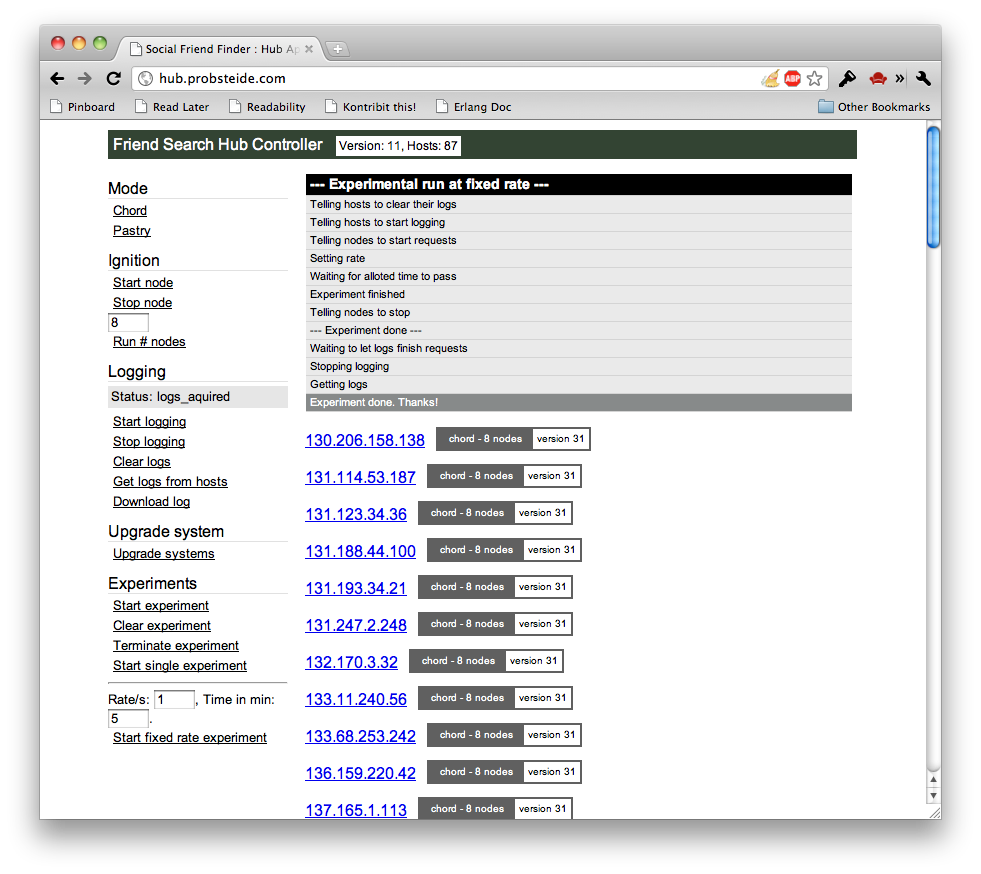
\includegraphics[width=0.9\linewidth]{illustrations/HubApp.png}
\caption{The Hub Application interface. A bare-bones web application that allows me to start and stop nodes, change between using Chord and Pastry, and start and stop experiments}
\label{hubApp}
\end{center}
\end{figure}


\subsection{Distributed Hash Tables - 101}
% How DHT's work
% * Quick intro, what will discuss
% *   For each item how Chord and Pastry differ

In this section I will briefly introduce the concept of Distributed Hash Tables. I will then go on to describe how the keyspace is organized and how it is divided amongst nodes participating in a Distributed Hash Table. After that we will look at how Pastry and Chord nodes route messages through their networks.

\mbox{}

% * What is a Dht?
Loosely defined, a Distributed Hash Table is a set of independent entities that have agreed to collectively store and make available a set of data items accessible under keys that fall into a well defined keyspace. Each such entity is generally called a node. 

By design, each node participating in the Distributed Hash Table only needs to know about a subset of the other nodes in the network. By carefully choosing which other nodes a given node knows about, any one node can reach any of the other nodes in a bounded number of hops.
How this is actually done will be discussed shortly.

% * What is the responsibility of a node?
% *   How is keyspace divided up
The keyspace is numeric and ranges from 0, and in the case of my implementations of Chord and Pastry, to $2^{160} - 1$. It wraps around at the boundaries so that 0 is immediately following $2^{160} - 1 $. It can be useful to think of the keyspace as a circle.

Each node is identified by a key. This key is in the same keyspace as the keys for the data stored in the Distributed Hash Table. In one sense nodes are just a special kind of data.

Each node is responsible for a part of the keyspace. All data items with keys in this key segment are stored by that particular node. For this reason it is important that the keys of both the nodes and the data are uniformly spread in the keyspace, so the amount of data stored by any one node is inverse proportional to the number of nodes in the Distributed Hash Table. This in achieved by using strong hash functions. In the case of my implementations I use SHA (FIPS 180-2).

\begin{figure}[!htb]
\begin{center}
	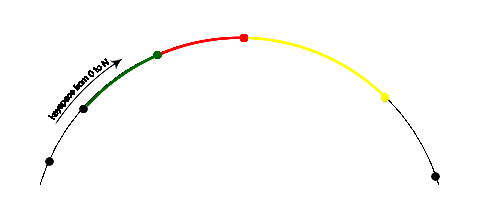
\includegraphics[width=0.9\linewidth]{illustrations/ChordKeySpace.eps}
  \caption{Illustration of how the keyspace is divided between Chord nodes.}
  \label{keyspaceChord}
\end{center}
\end{figure}

\begin{figure}[!htb]
\begin{center}
	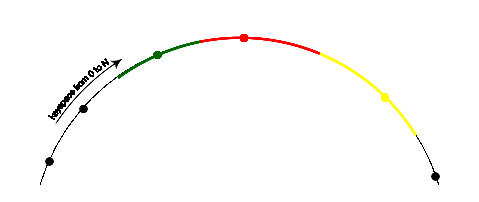
\includegraphics[width=0.9\linewidth]{illustrations/PastryKeySpace.eps}
  \caption{Illustration of how the keyspace is divided between Pastry nodes.}
  \label{keyspacePastry}
\end{center}
\end{figure}

The way in which the subsets of the keyspace is associated with nodes differs slightly between Chord and Pastry. In Chord, a node is responsible for all keys in the range of its predecessors and up to and including itself. In Pastry on the other hand all keys numerically closer to a node than to its neighbour is the responsibility of that particular node. The Chord approach is somewhat easier to implement, but other than that they seem equally well suited for the task.

% * How are the routing tables organized?
% *   What information is stored
% *   How is a message routed from A to B?
% *   How is a key lookup done?

Now that we have discussed how the keyspace is split among nodes in a Distributed Hash Table I will discuss what routing information is required and how messages are actually routed from an origin to a destination. This is the area in which Chord and Pastry differ the most.

\paragraph{The Chord approach to routing}
The Chord routing table is designed in such a way that a node knows many more nodes immediately following it in the keyspace than it does nodes further away. Additionally each node maintains a list of its immediate successors and a pointer to its predecessor in the keyspace.

Whenever a key lookup is performed, the node performing the lookup asks the node in its routing table most closely preceding the target key whether they know about a node closer to the key that still precedes it. If it does, the node performing the lookup in turn asks this node if it knows a closer but preceding node. Once the node immediately preceding the key has been found, its successor is taken as the authority for that particular key.
The data for the key, if present in the network, will be stored by that particular node.
By always asking for the node most closely preceding the target key, we are guaranteed never to overshoot the node responsible for it.

A Chord network works correctly as long as all nodes at all times know who their immediate successor is. If nodes \emph{only} knew about their successor, a key-lookup would necessarily have to do a linear search amongst all the nodes. While this would work it is not efficient. Instead each node maintains a routing table so it has information about nodes further away in the network as well. By design this routing table is such that in a network where all the routing tables are correctly maintained, the number of hops needed are bounded by the logarithm of the number of nodes in the network.


\paragraph{The Pastry approach to routing}
Pastry interprets keys as numbers in some arbitrary base b.
Each node maintains a routing table with an entry per digit in its own key. Each entry represent nodes with keys sharing all the digits up to that particular digits.
When routing a message it is always forwarded to a node that shares \emph{at least} as many digits with the key as the current node does, but additionally is numerically closer to the key. If there is no such node in the routing table, the node checks a table of its immediate neighbours to see if the respective key is in their range. If the given node is the node with a key numerically closest to the message key, the message has arrived at its destination, and is handed over to the Pastry Application.

The number of hops a message has to take is nicely bounded by the parameter b.

\paragraph{Differences between Chord and Pastry}
When constructing and maintaining its routing tables, Pastry uses a proximity heuristic to favour nodes closer to itself. This proximity measure can be anything from latency to the number of routing hops to geographical proximity. Ideally this heuristic should honour the triangle inequality, but in reality this isn't always easy to achieve. In my case I am using the number of routing hops in the actual network topology as a measure. This measure certainly does not honour the triangle inequality, but still seems to offer good performance.

Pastry also maintains a list of nodes that are its neighbours in terms of the proximity metric. These neighbours act as a low cost set of nodes to exchange routing information with.

To what extent these proximity heuristics improve the routing performance will be examined in the evaluation chapter.

\mbox{}

% * Summary
In this section we discussed how the key space is constructed and divided between nodes in Chord and Pastry, and also how Chord and Pastry respectively use their routing tables to route messages to the node responsible for the message key. We also looked at how Pastry uses an additional proximity measure to preferentially route messages through nodes closer to it.

%   How it all fits together

\subsection{Supervision in the context of my project}
In this section I will briefly discuss a key aspect of developing applications in Erlang: The use of supervisors to control application lifetime behaviour.

\begin{figure}[!htb]
\begin{center}
	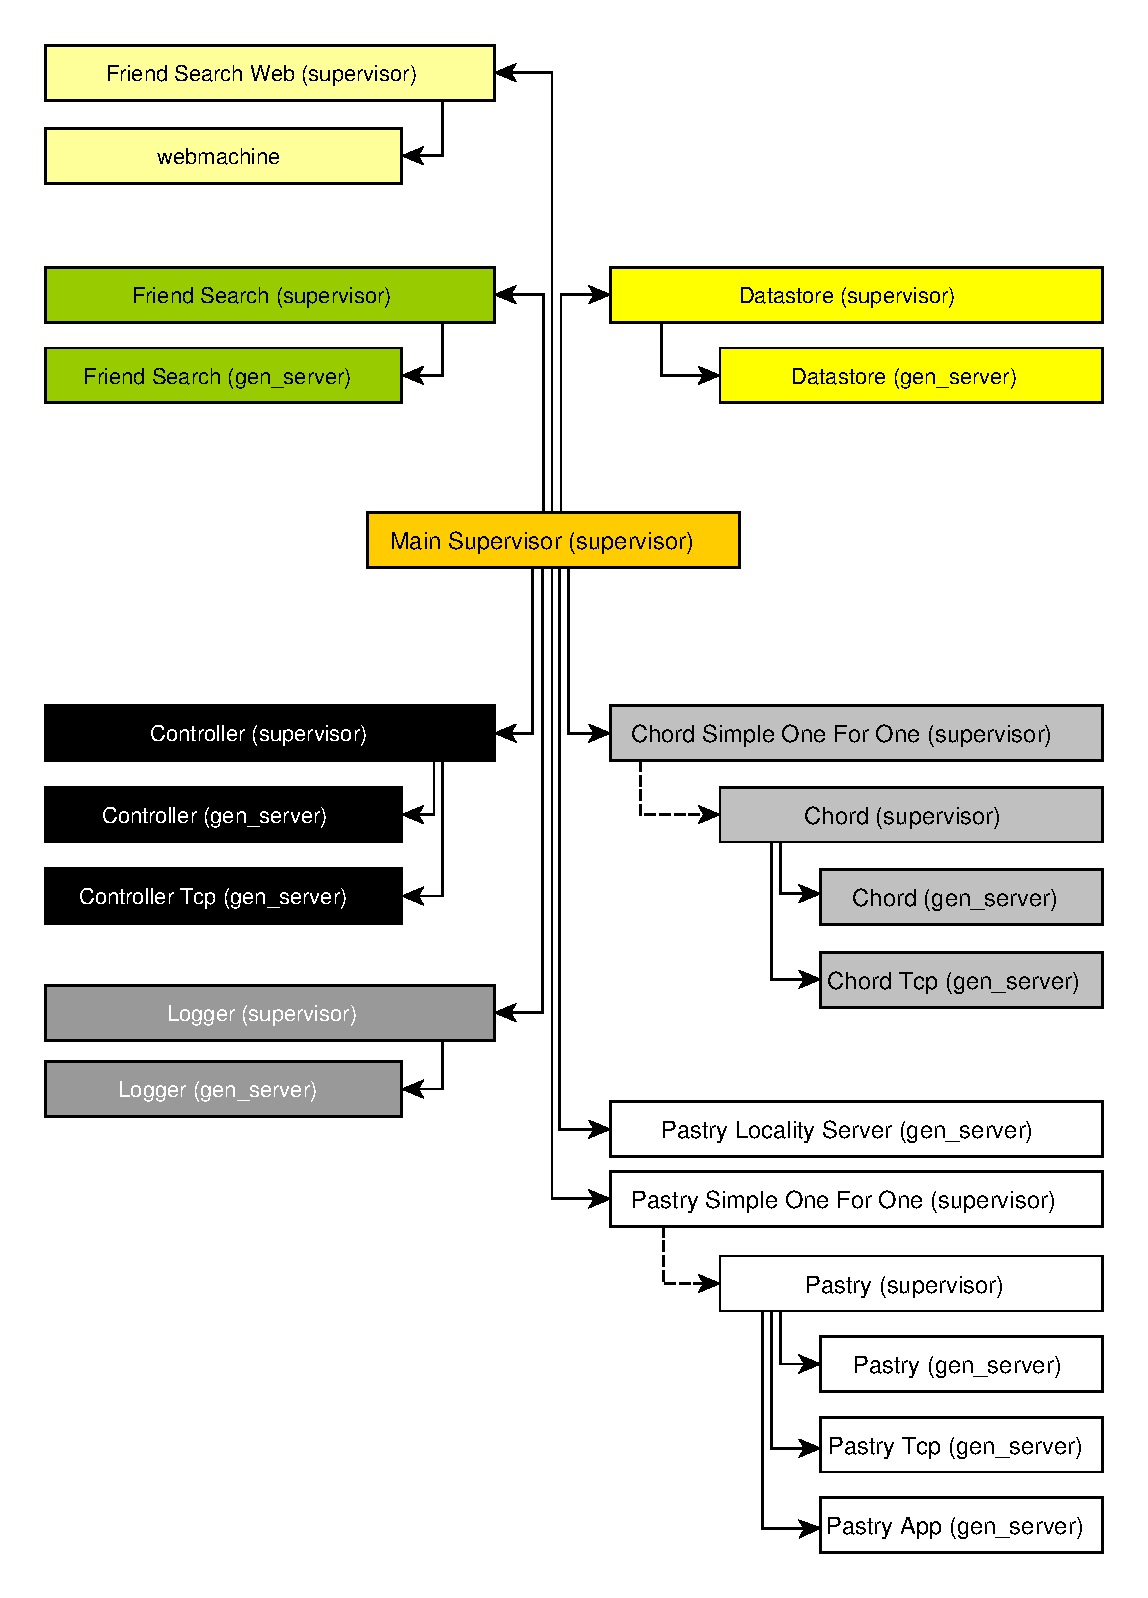
\includegraphics[width=0.9\linewidth]{illustrations/ClientSupervisionTree.eps}
  \caption{This figure shows the same main components as the component diagram shown earlier. It additionally shows the supervisors and gen servers that make up the application.}
  \label{supervisionTree}
\end{center}
\end{figure}

% * The use of supervisors
First let me introduce the concept of supervisors:
Supervisors are processes that are responsible for starting components of an application. For the lifetime of the component they monitor it. If it should fail the supervisor restarts it.

A supervisors supervisees are generally called its children. A supervisor can either have a single child or several children. In the case of supervisors with several children one has to distinguish between supervisors who restart all their children when one fails (one for all), or supervisors only restarting the child that died (one for one). Both types are used in my application. 

I want to introduce one last kind of supervisor that plays a crucial role in my application. It is called a Simple One For One supervisor (simple one for one). A Simple One For One Supervisor specialises in one particular type of children, but has the ability to start and stop arbitrary number of these children at will during the lifetime of the application. This in contrast to regular supervisors who only maintain a predefined set of children. I use this feature to enable the application controller to start and stop Chord and Pastry nodes at runtime.

One last thing we need to know before examining how supervisors are used in my application, is that one can build hierarchies of supervisors.

% * Different types of supervisors
% * What do I use where and why
% * Look at the overall supervision hierarchy of Search Application.
Now let us take a look at the supervision tree of the search application shown in Figure \ref{supervisionTree}.
The main components are the same as in the component overview shown in Figure \ref{figComponents}.

Please take a particularly close look at the Pastry branch of the diagram. The Pastry Simple One For One supervisor only knows about one kind of child: the Pastry Supervisor. The Pastry supervisor in turn knows how to start the main Pastry server component, but also starts the Pastry Tcp component which is the communication component of the Pastry node, and the Pastry Application that is responsible for handling message delivery and storage. The Pastry Supervisor coincidentally is a \emph{one for all} supervisor. When any of its children die, the ones that are alive are also terminated before they are collectively restarted. I decided on this approach as the components are tightly intertwined and rely on a particular instance of the application running.

The Chord branch very much resembles that of Pastry. 

All the other supervisor-child pairs use a \emph{one for one} restart policy.

\mbox{}

We have now seen how supervisors play a crucial part in the design and structure of my project, and how most importantly \emph{simple one for one} supervisors give the flexibility of starting and stopping an arbitrary number of children giving us the flexibility of running an arbitrary number of Chord and Pastry nodes on a single server, and adjusting that number at runtime.

\subsection{Summary of the implementation chapter}
In this chapter we discussed what data is stored in the Distributed Hash Tables, how we got around the difficulties of efficiently searching through a key-value store. We also discussed the negligible additional storage cost of using link records in addition to profile records, and the less negligible overhead of potentially having to resolve a multitude of link records during search.

We looked at what third party libraries have been used, and how test-driven development played a significant role in the development of my project.

We discussed the different main components of the search system, how Chord and Pastry perform key-lookups in their networks and their main differences.

Lastly we also discussed how the Erlang concept of process supervisors plays a role in modularising the code and restarting failing processes.

In the next chapter I will discuss how I evaluated my project and how the performance of Chord and Pastry compare.

